\documentclass[tikz, dvipsnames]{standalone}


\usepackage{pgfplots}


\begin{document}
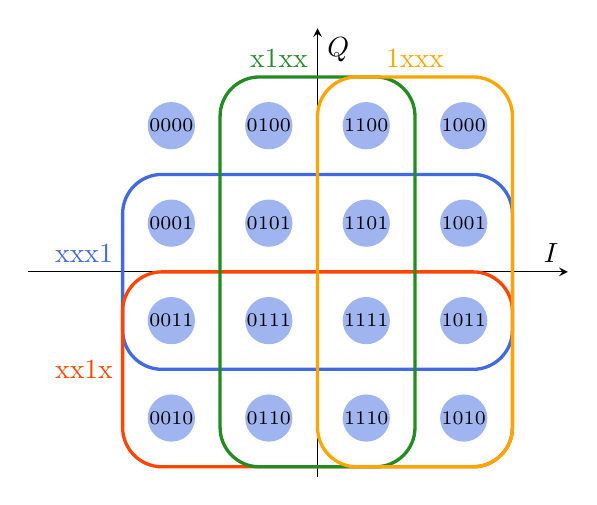
\begin{tikzpicture}[node/.style={circle,fill=RoyalBlue!50!White, inner sep=0pt,minimum size=6mm}]
\begin{axis}[axis lines=middle,
xmin=-5,
xmax=4.2,
ymin=-4.2,
ymax=5,
axis equal,
xlabel=$I$,
ylabel=$Q$,
clip=false,
xticklabels=\empty,
yticklabels=\empty]

\node[node] at (axis cs:-3,3)  {\scriptsize 0000};
\node[node] at (axis cs:-1,3)  {\scriptsize 0100};
\node[node] at (axis cs:1,3)   {\scriptsize 1100};
\node[node] at (axis cs:3,3)   {\scriptsize 1000};
\node[node] at (axis cs:-3,1)  {\scriptsize 0001};
\node[node] at (axis cs:-1,1)  {\scriptsize 0101};
\node[node] at (axis cs:1,1)   {\scriptsize 1101};
\node[node] at (axis cs:3,1)   {\scriptsize 1001};
\node[node] at (axis cs:-3,-1) {\scriptsize 0011};
\node[node] at (axis cs:-1,-1) {\scriptsize 0111};
\node[node] at (axis cs:1,-1)  {\scriptsize 1111};
\node[node] at (axis cs:3,-1)  {\scriptsize 1011};
\node[node] at (axis cs:-3,-3) {\scriptsize 0010};
\node[node] at (axis cs:-1,-3) {\scriptsize 0110};
\node[node] at (axis cs:1,-3)  {\scriptsize 1110};
\node[node] at (axis cs:3,-3)  {\scriptsize 1010};


\draw[rounded corners=5mm, RoyalBlue, very thick] (axis cs:-4,2) rectangle (axis cs:4,-2);
\node[anchor=south east,RoyalBlue] at (axis cs:-4,0) {xxx1};

\draw[rounded corners=5mm, OrangeRed, very thick] (axis cs:-4,0) rectangle (axis cs:4,-4);
\node[anchor=east,OrangeRed] at (axis cs:-4,-2) {xx1x};

\draw[rounded corners=5mm, ForestGreen, very thick] (axis cs:-2,4) rectangle (axis cs:2,-4);
\node[anchor=south east,ForestGreen] at (axis cs:0,4) {x1xx};

\draw[rounded corners=5mm, Orange, very thick] (axis cs:0,4) rectangle (axis cs:4,-4);
\node[anchor=south,Orange] at (axis cs:2,4) {1xxx};



\end{axis}
\end{tikzpicture}
\end{document}